% This is samplepaper.tex, a sample chapter demonstrating the
% LLNCS macro package for Springer Computer Science proceedings;
% Version 2.21 of 2022/01/12
%
\documentclass[runningheads]{llncs}
%
\usepackage[T1]{fontenc}
% T1 fonts will be used to generate the final print and online PDFs,
% so please use T1 fonts in your manuscript whenever possible.
% Other font encondings may result in incorrect characters.
%
\usepackage{graphicx}
% Used for displaying a sample figure. If possible, figure files should
% be included in EPS format.
%
% If you use the hyperref package, please uncomment the following two lines
% to display URLs in blue roman font according to Springer's eBook style:
%\usepackage{color}
%\renewcommand\UrlFont{\color{blue}\rmfamily}
%\urlstyle{rm}
%
\begin{document}
%
\title{Reducing Intuitive-Physics Prediction Error through Playing}
%
\titlerunning{Reducing Prediction Error through Playing}
% If the paper title is too long for the running head, you can set
% an abbreviated paper title here
%
\author{Olivier L. Georgeon\inst{1, 2}\orcidID{0000-0003-4883-8702} \and
Paul Robertson\inst{3}\orcidID{0000-0002-4477-0379} }
%
\authorrunning{Georgeon and Robertson}
% First names are abbreviated in the running head.
% If there are more than two authors, 'et al.' is used.
%
\institute{UR CONFLUENCE: Sciences et Humanites (EA 1598), UCLy, France 
	\email{ogeorgeon@univ-catholyon.fr} \and
SyCoSMA, LIRIS, CNRS, Villeurbanne, France \and
DOLL Labs, Lexington, MA, USA\\
\email{paulr@dollabs.com}}
%
\maketitle              % typeset the header of the contribution
%
\begin{abstract}
We present a method for an autonomous robot to generate behaviors to calibrate its intuitive-physics engine also known as the ``Game Engine in the Head'' (GEITH).
%The robot selects behaviors that yield information to refine the GEITH parameters. 
At the beginning of each interaction cycle, the robot uses its GEITH to run a simulation to compute predicted sensory signals. 
For each sensor, prediction error is the difference of the predicted sensory signal minus the actual sensory signal received at the end of the interaction cycle. 
Results show that over a few tens of interaction cycles, the robot improves its GEITH calibration and decreases its prediction errors. 
Moreover, the robot generates behaviors that human observers describe as playful.

\keywords{Active infernce  \and constructivist learning \and enaction \and intrinsic motivation \and robotics \and core knowledge.}
\end{abstract}
%
%
%
\section{Introduction}
\label{sec:intro}

It is widely believed that cognitive beings possess some kind of a \textit{world model} that they use to generate intelligent behaviors.
How they construct, maintain, and use this world model remains, however,  an open question in cognitive science and artificial intelligence. 

The Partially Observable Markov Decision Process (POMDP) literature has proposed a broad range of methods to infer a \textit{belief state} in a partially observable process.
The belief state amounts to the agent's world model of the environment that the agent can only partially observe.  
If the state transition function and the observation function are known \textit{a priori}, the problem of computing the belief state has been mathematically solved \cite{astrom1965optimal}. 
It was, however, also proven that the implementation of the solution becomes intractable as the set of states and observation grows. 
%Without knowledge of the state transition and observation functions, the problem of inferring belief states in POMDPs does not lend itself to a mathematical analysis. 

Karl Friston and his research group have proposed Active Inference \cite[e.g.]{smith_step-by-step_2022} as a method to interactively refine the world model by minimizing \textit{free energy}, or equivalently, prediction error and surprise \cite{friston_free-energy_2010}.
The world model %at step $t$ 
is represented as the distribution of probability %$\mu_t$ that gives the probability 
of each possible state of the world. 
In essence, at each instant, the agent estimates which states are the most or least likely to be the actual state of the world.
%$s \in S$ of all the possible states of the world. 
%This method iteratively updates $\mu_t$ on each interaction cycle.
%The agent selects the action that is expected to maximize the information gained to refine the probability distribution. 
%The estimation of expected information gained is computed through the variational free energy which involves a divergence between two probability distributions: the agent's world model $\mu$ and the joint probability distribution $g = P(O, S)$ of observations $O$ and world states $S$ called the \textit{generative model}. 
This method, however, requires that the set of all world states %$S$ 
be known \textit{a prior}, which is not the case of robots in the open world.
The relations between states and observations must also be known \textit{a priori}, which we prefer to avoid.
Moreover, computing the free energy remains too computationally intensive for our robotics experiment.
%remain; however to  and the high number of interaction cycles to converge to a useful world model makes this method inapplicable in our case of a robot interacting with the open world. 

The POMDP and active inference literature led us to hypothesize that inferring the world model through experience of interaction requires prior assumptions to reduce complexity \cite{georgeon_artificial_2024}. 
The present study examines how the ``Game Engine In The head'' (GEITH) can work as a suitable prior assumption that an autonomous robot could use to reduce its prediction errors. 

Joshua Tenenbaum and his research group have proposed the GEITH \cite{battaglia_simulation_2013} as the capacity of cognitive beings to simulate basic dynamics of physics and interactions. 
In mammals, the GEITH would rest upon brain structures that are partially predefined by genes and then completed through ontogenetic development.  
Similarly, it is possible to endow artificial agents and robots with a predefined software game engine, and expect them to refine the parameters of their game engine as they test their predictions in the world.

This paper proposes an approach to designing autonomous agent that can refine their GEITH through their lifetime.
The refinement of the game engine is measured through two methods. 
The first is performed by the robot itself by measuring the prediction error of sensory signals. 
Decrease in prediction errors shows improvement of the game engine. 
The second is performed by the experimenter by assessing whether the game engine parameters converge towards a target range that indicates that the robot managed to calibrate its GEITH. 




\section{Our hypothesis}

We comply with active inference theory in several regards. 
Firstly, we do not consider sensory signals to be \textit{representational} of the environment's state. 
Different sensory signals may come out of the same environment state depending on the agent's action. 
This implies a ``conceptual inversion'' of the interaction cycle in which action comes first and sensory signal comes second as an  \textit{outcome} of action. 
Secondly, we do not provide the agent with presupposed ontological knowledge about entities in the environment. 
The agent must infer the existence and properties of entities by itself through patterns of interactive experience. 
This view can be tracked back to Whitehead's process philosophy in which phenomenal experience involves abstracting entities out of events \cite{whitehead1929}. 
Thirdly, no extrinsic goal is encoded in the agent in the form of goal states that the agent should search based on reward or other criteria. 
We nonetheless accept to associate some \textit{prior preference valences} with interactions. 
In short, the agent has no \textit{rewarding world states} but has \textit{rewarding interactions} (positive or negative).
For a deeper examination of these principles in relation with the active inference literature, we refer the reader to our previous article \cite{georgeon_artificial_2024}.

We also adopt \textit{prediction error} as a measure of the quality of the agent's world model. %, and minimizing surprise is a powerful motivator. 
%Indeed, to survive, cognitive beings should avoid bad predictions as much as they can. %generally stay away from bad surprises.
As introduced in Section \ref{sec:intro}, however, we are not using gradient descent of prediction error (or surprise) as a motivational principle to drive the learning process. 
As we will develop, our agent is not always driven by a value optimization process; it may sometimes enact selfless behaviors.
% We are investigating an alternative approach based on an innate set of behaviors that the robot may select depending on its \textit{emotional state}.  
For us, prediction-error reduction is not a means to improve the world model but a consequence of its improvement.

We are using a cognitive architecture that we designed previously based on sensorimotor and enactive principles \cite{georgeon_artificial_2024}. 
The present article reports the integration of the new GEITH module within this cognitive architecture as illustrated in Figure \ref{fig:geith}. 
The GEITH supports the simulation of interactive behaviors before their selection by the cognitive architecture and their enaction by the robot. 
At the beginning of each interaction cycle, the simulation computes the \textit{predicted outcome}.
At the end of the interaction cycle, the predicted outcome is compared with the \textit{actual outcome} to compute the prediction error.   
We investigate the core elements of the GEITH that are needed for the agent to reduce prediction error. 

We draw inspiration from studies on \textit{core knowledge} in the brain of animals and human infants. 
For example, Elizabeth Spelke and her colleagues argued for the existence of two core systems of geometry that ``evolved before the emergence of the human species'':  
``The \textit{core navigation system} captures absolute distance and sense [..] but not relative length or angle; the \textit{core form analysis system} does the reverse'' \cite[p. 2789]{spelke_core_2012}.
We start by implementing the minimal requirements she deems necessary for both systems, namely the ability to handle points and lines in spatial memory, the foundational elements of Euclidean geometry. 

Our cognitive architecture encodes behaviors as \textit{composite interactions} which are sequences of \textit{primitive interactions}.
A primitive interaction is a specification of a \textit{control loop} that involves actuator commands, expected sensory feedback, spatio-temporal attributes, termination conditions, termination outcome, and preference valence. 
Examples are in Section \ref{sec:expe}. 
The GEITH may consider some outcomes as resulting from the interaction with ``something'' in the environment.
In this case, the GEITH instantiates a data structure called a \textit{phenomenon}\footnote{Common-sense usage of the term \textit{phenomenon}: ``something'' that a cognitive being perceives in the environment. Technically: ``any useful grouping of a subset of spatio-temporal patterns experienced by an agent in an environment'' \cite[p. 8]{thorisson_explanation_2021}.} and localizes this phenomenon at the position of the interaction in spatial memory.
Next, the GEITH simulates subsequent interactions with phenomena to predict future outcomes. 
The present study focuses on the simplest possible kind of phenomenon: points on the two-dimensional floor.

We seeded the cognitive architecture with ``innate'' composite interactions (Fig. \ref{fig:geith}, top-center) that cause the robot to explore the environment and to interact with points encountered on the floor. 
Here we do not examine the learning of new composite interactions (we did in other studies \cite{georgeon_cash_2019}) but only the refinement of the GEITH parameters to reduce prediction error.
The cognitive architecture uses variables that represent the robot's \textit{emotional state} to selects composite interactions to try to enact.

We use Hugo Lövheim's ``cube of emotions'' \cite{lovheim_new_2012} as a basic emotional model based on three neurotransmitters: dopamine (DA), serotonin (5-HT), and nor-adrenaline (NA) (Fig. \ref{fig:geith}, top right).
This model associates dopamine with pleasure and reward-seeking behavior, serotonin with well-being and playful behavior, and nor-adrenaline with arousal and stress responses.
It has been successfully used for simple emotional robotics.
Our robot visually indicates its predominant neurotransmitter level using an intuitive color code developed by Max Talanov and his team: green for dopamine, white for serotonin, red for noradrenaline, and blue when all three neurotransmitter levels are low \cite{chebotareva_emotional_2019}.

The GEITH implements two levels of spatial working memory: \textit{egocentric} and \textit{phenomenon-centric} (Fig. \ref{fig:geith}, center).  
The robot's displacements are tracked in the egocentric reference frame using an Inertial Measurement Unit that plays a similar role as the vestibular system. 
Using spatial-displacement information, the GEITH updates the position of the recent history of interactions in egocentric memory (Fig. \ref{fig:video}, top right).
When the robot encounters a new phenomenon, the GEITH instantiates a new reference frame centered on this phenomenon to track the displacement of the robot relative to this phenomenon (Fig. \ref{fig:video}, bottom right). 
This mechanism of coordinate conversion relates to that implemented by Howard Schneider's in his Causal Cognitive Architecture \cite{schneider_enabling_2020}, and to 
Jeff Hawkins' thousand brain hypothesis \cite{hawkins_framework_2019} according to which the brain records thousands of small spatial models to memorize interactions with different kinds of objects.
We implemented Tenenbaum's idea to give a \textit{sleep}/\textit{awake} attribute to phenomena. If the GEITH detects that the phenomenon moves, it switches the attribute to \textit{awake}.

As we shall see in the experiment presented next, prediction errors may have a variety of causes sometimes difficult to untangle. 
Again, we are looking for core systems of causal explanation that may have evolved in the brain.
The literature has pointed out that explanation requires isolating relevant elements of context, and tracking their transformation through series of events \cite{thorisson_explanation_2021}. 
Explanation may also involve a confrontation between proponent and opponent arguments, and interaction with the world to arbitrate. 

\begin{figure}
	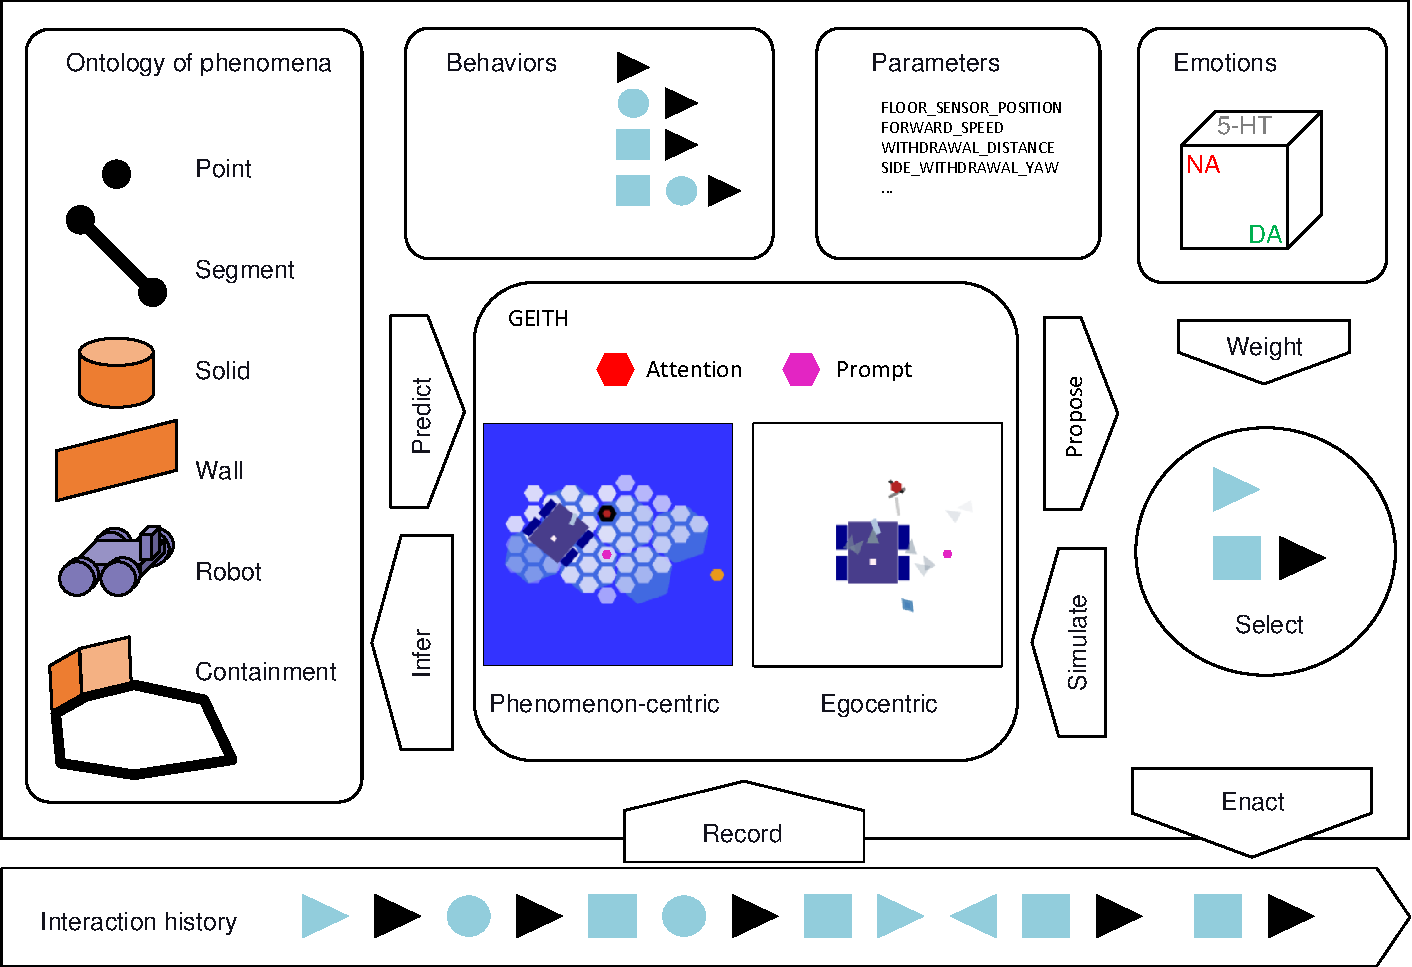
\includegraphics[width=\textwidth]{Figure_geith.pdf}
	\caption{The game engine within the robot's cognitive architecture.
	Bottom: the history of interactions enacted over time.
	Center: the working memory that implements the game engine and proposes future behaviors.
	Left: the types of phenomena inferred trough interactive experience.
	Top center: set of behaviors.
	Top right: The three-dimensional emotional state based on dopamine (DA), serotonin (5-HT), and nor-adrenaline (NA) levels.
	Right: the decider selects the next behavior based on the emotional state and the expected outcome predicted from simulation.} \label{fig:geith}
\end{figure}



\section{Experiment}
\label{sec:expe}

We designed a robotic platform called Petitcat\footnote{In this section, we personalize the robot by its name Petitcat and the pronoun ``he''. We do not claim that he has a psychology, let alone a gender, but this way if speaking feels more natural to human experimenters and some readers.} based on the ``robot car'' commercialized by Osoyoo \cite{osoyoo_robot_car}.
%For this experiment, 
We added an Inertial Measurement Unit (IMU) and an RGB LED as the emotion indicator (Fig. \ref{fig:video}). 

\begin{figure}
	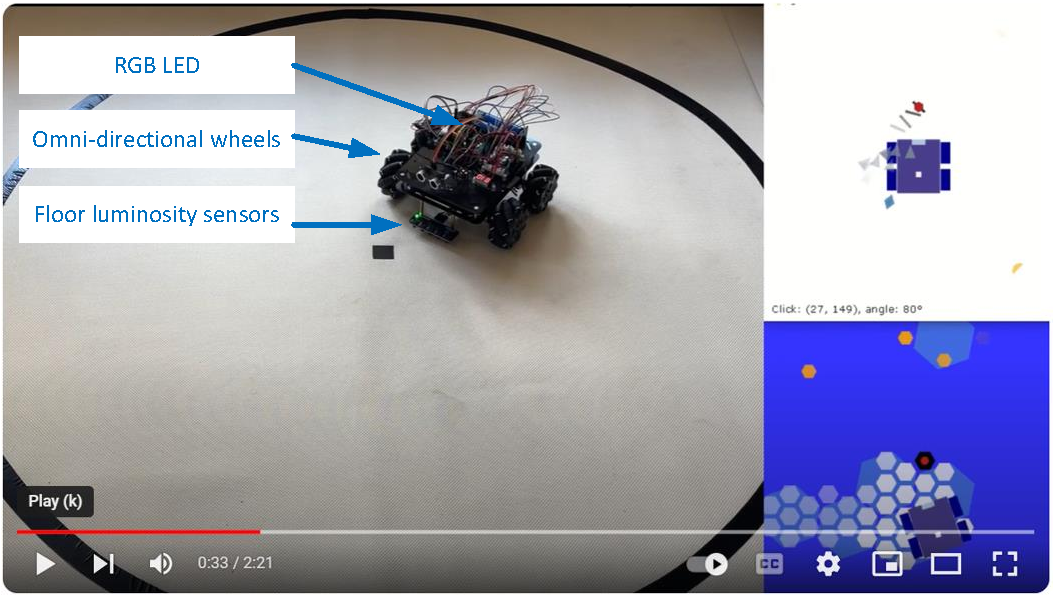
\includegraphics[width=\textwidth]{Figure_video.pdf}
	\caption{Screenshot of a video example run \cite{georgeon_petitcat_2024}.
		Left: Petitcat playing with a point on the floor.
		Top right: Petitcat's egocentric memory. Black segments: black point detection events. 
		Bottom right: allocentric memory. Black hexagon: the black point used as a point of reference. Yellow hexagons: echo measured with the sonar. Red hexagon: the robot's focus of attention.} \label{fig:video}
\end{figure}

The C++ software running on the Arduino board controls the enaction of primitive interactions. 
A personal computer implements the GEITH and the cognitive architecture that remote controls the robot through wifi.
The cognitive architecture selects the primitive interaction to try to enact and sends it to the robot. 
The robot tries to enact it and sends the outcome back to the PC.  
The code is open source and shared online \cite{petitcat_github}.

For this experiment, we defined four possible commands: \texttt{forward}, \texttt{backward}, \texttt{swipe}, and \texttt{turn}. 
\texttt{Turn} consists in turning in place. Its spatio-temporal attribute is the target yaw (float), negative when counter-trigonometric. 
\texttt{Swipe} is a lateral translation. Its spatio-temporal attributes are the direction (left or right) and target duration (float). 
\texttt{Forward} and \texttt{backward} are longitudinal translations. Their spatio-temporal attribute is the target duration (float).   
%they have been separated rather than using a direction attribute because they are conceptually different: moving toward or away from a target. 

The control loop monitors the luminosity of the floor, the yaw, and the distance of echo signals during the enaction of interactions. 
The termination conditions of the primitive interactions are reaching the target yaw or duration, or detecting a black tape on the floor, making two possible outcomes: \texttt{tape} or \texttt{no\_tape}, which gives eight primitive interactions (4 commands $\times$ 2 outcomes).
All interactions were given a null prior valence except $\langle$\texttt{forward}, \texttt{no\_tape}$\rangle$ that has a positive one.
Additionally, the robot returns the measured spatial attributes to the GEITH: measured duration (float), measured yaw (float), and the direction of the black tape detection if any (none, left, front, right). 

When the black tape is detected, a ``reflex'' movement is performed to withdraw away from the tape by a few centimeters. 
When the detection is on the side, this withdrawal includes a rotation to the opposite side, which tends to bring the robot back into a position perpendicular to the tape.

We seeded the cognitive architecture with the four ``playful'' composite interactions below. 
The GEITH tries to simulate them, computes their spatio-temporal attributes, and proposes those that are feasible in the current context.
\begin{enumerate}
	\item $\langle\langle$\texttt{forward}, \texttt{tape}$\rangle\rangle$
	\item $\langle\langle$\texttt{turn}, \texttt{no\_tape}$\rangle\langle$\texttt{forward}, \texttt{tape}$\rangle\rangle$
	\item $\langle\langle$\texttt{swipe}, \texttt{no\_tape}$\rangle\langle$\texttt{forward}, \texttt{tape}$\rangle\rangle$
	\item $\langle\langle$\texttt{swipe}, \texttt{no\_tape}$\rangle\langle$\texttt{turn}, \texttt{no\_tape}$\rangle\langle$\texttt{forward}, \texttt{tape}$\rangle\rangle$. 
\end{enumerate}

When the actual outcome differs from the expected outcome, the tentative enaction of the primitive interaction is considered a failure and the enaction of the composite interaction is interrupted. 
This happens either when the GEITH predicted a tape detection that did not happen or the reverse. 

The levels of all three neurotransmitters can vary from 0 to 100 and are initialized at 50 (DA prevails in case of draw).
Prevalence of DA makes Petitcat initially select the \texttt{forward} interaction because it has a positive valence.
When he detects a point, 5-HT increases to MAX-5-HT. Prevalence of 5-HT triggers the selection of playful interactions with this point.
On each playful interaction, if the prediction errors do not decrease (i.e., prediction does not improve), 5-HT decreases by 1.
When 5-HT decreases below or equal to DA, the  $\langle$\texttt{forward}, \texttt{no\_tape}$\rangle$ interaction is again selected meaning that Petitcat disinterests from the point and goes exploring new destinations. 
During play, when Petitcat unexpectedly fails to detect the point, NA increases to MAX-NA, which causes the selection of \texttt{search} behaviors. 
DA then decreases of 1 on each interaction or is reset to MIN-NA when Petitcat finds the point again.  



% \subsection{The robotics platform}

% \subsection{The Game Engine In The Head}

\section{Results}

Several videos are available online. 
Here we analyze a representative run recorded on video \cite{georgeon_petitcat_2024}.

\begin{figure}
	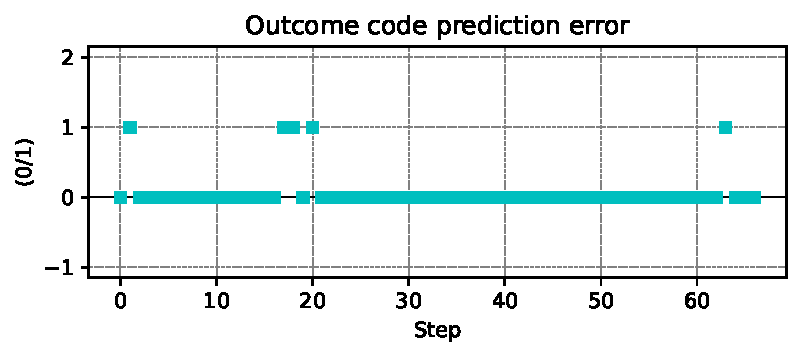
\includegraphics[width=\textwidth]{01_Outcome_code.pdf}
	\caption{Prediction error of black phenomenon detection.
	Step 2: the robot did not expect to detect the point.
	Steps 17: the robot expected to detect the point while translating forward but missed it.
	Steps 18: the robot expected to not detect the point while turning around but detected it.
	Step 20: the robot did not predict detecting the point through simulation but it did. 
	Step 65: The robot did not expect to detect the surrounding arena. } \label{fig:yaw_pe}
\end{figure}

\begin{figure}
	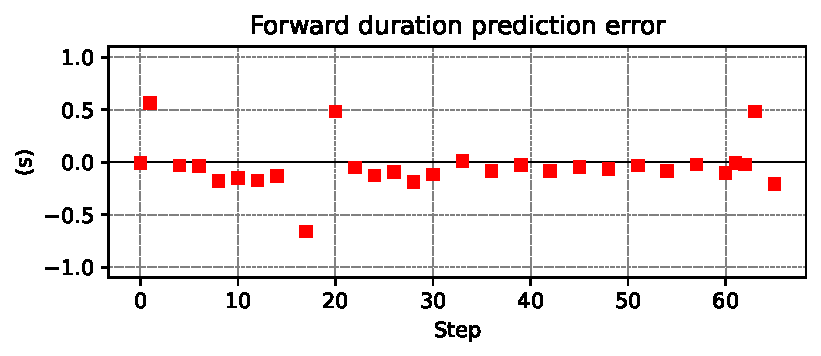
\includegraphics[width=\textwidth]{07_Forward_duration_pe.pdf}
	\caption{Move forward duration prediction error.
	Step 2 and 20: the forward translation was unexpectedly interrupted by the point detection.
	Step 17: the forward duration was longer than expected because the robot did not detect the point.
	From Step 21 to 64: forward duration prediction error slightly decreases. 
	Step 65: the forward translation was unexpectedly interrupted by the detection of the arena border.} \label{fig:yaw_re}
\end{figure}


\begin{figure}
	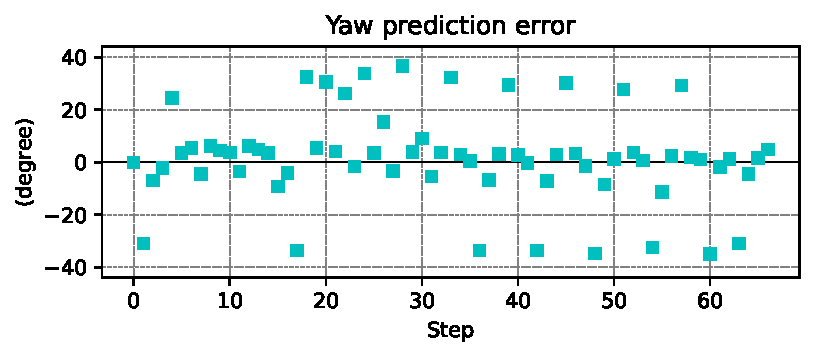
\includegraphics[width=\textwidth]{02_yaw_pe.pdf}
	\caption{The yaw prediction error shows no significant trend when we do not distinguish between the different kinds of interactions.} \label{fig:yaw_pe}
\end{figure}

\begin{figure}
	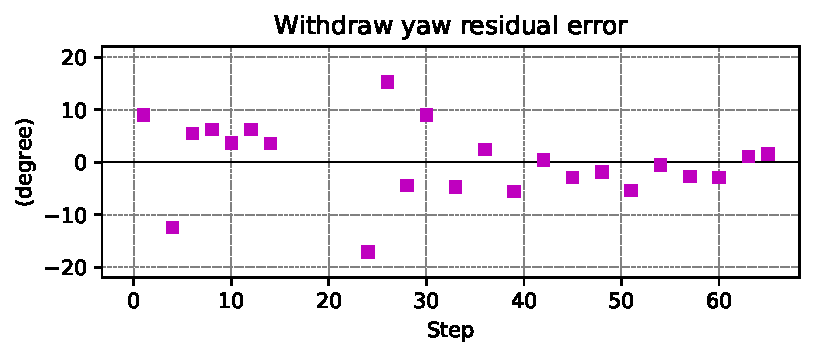
\includegraphics[width=\textwidth]{03_yaw_re.pdf}
	\caption{The yaw residual error during interactions in which the robot detects the point decreases significantly after Step 26.} \label{fig:yaw_re}
\end{figure}

\begin{figure}
	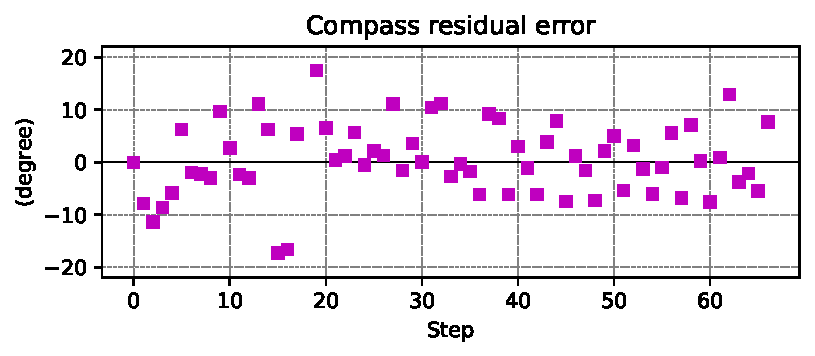
\includegraphics[width=\textwidth]{04_Compass.pdf}
	\caption{The compass residual error decreases after step 20 when the robot starts circling around the point.
	It nonetheless remains noisy due to sensor imprecision.
	The sliding average over 10 interactions tends to 0.8° and the standard deviation to 7.4°.} \label{fig:compass}
\end{figure}

\section{Conclusion}

We are not claiming the robot can actually \textit{experience} emotions let alone have sentience. 
His internal model of emotions, nonetheless, helps generate behaviors that human observers easily interpret as lifelike. 
The emotional indicator facilitates this interpretation. 

\begin{credits}

%\subsubsection{\ackname} A bold run-in heading in small font size at the end of the paper is
%used for general acknowledgments, for example: This study was funded
%by X (grant number Y).

%\subsubsection{\discintname}
%It is now necessary to declare any competing interests or to specifically
%state that the authors have no competing interests. Please place the
%statement with a bold run-in heading in small font size beneath the
%(optional) acknowledgments\footnote{If EquinOCS, our proceedings submission
%system, is used, then the disclaimer can be provided directly in the system.},
%for example: The authors have no competing interests to declare that are
%relevant to the content of this article. Or: Author A has received research
%grants from Company W. Author B has received a speaker honorarium from
%Company X and owns stock in Company Y. Author C is a member of committee Z.
\end{credits}
%
% ---- Bibliography ----
%
% BibTeX users should specify bibliography style 'splncs04'.
% References will then be sorted and formatted in the correct style.
%
\bibliographystyle{splncs04}
\bibliography{georgeon.bib}
%
\end{document}
